\documentclass[letterpaper]{article}
\usepackage{amssymb}
\usepackage{fullpage}
\usepackage{amsmath}
\usepackage{epsfig,float,alltt}
\usepackage{psfrag,xr}
\usepackage[T1]{fontenc}
\usepackage{url}
%\usepackage{mathtools}

\begin{document}

\newcommand{\trace}{\mathrm{trace}}
\newcommand{\real}{\mathbb R}  % real numbers  {I\!\!R}
\newcommand{\nat}{\mathbb R}   % Natural numbers {I\!\!N}
\newcommand{\cp}{\mathbb C}    % complex numbers  {I\!\!\!\!C}
\newcommand{\ds}{\displaystyle}
\newcommand{\mf}[2]{\frac{\ds #1}{\ds #2}}
\newcommand{\book}[2]{{Luenberger, Page~#1, }{Prob.~#2}}
\newcommand{\spanof}[1]{\textrm{span} \{ #1 \}}
\parindent 0pt


\begin{center}
{\large \bf HW \# 06 Solutions}
\end{center}

\vspace*{1cm}

%Prob. 1 Matrices
\noindent \textbf{Problem  1:}
$$O = \left[\begin{array}{ccc} 
-\dfrac{1}{2} & \dfrac{\sqrt{2}}{2} & \dfrac{1}{2} \\[2ex]
-\dfrac{\sqrt{2}}{2} & 0 & -\dfrac{\sqrt{2}}{2} \\[2ex]
\dfrac{1}{2} & \dfrac{\sqrt{2}}{2} & -\dfrac{1}{2}
\end{array}\right] $$

$$\Lambda = \left[\begin{array}{ccc} 
2-\sqrt{2} & 0 & 0 \\
0 & 2 & 0 \\
0 & 0 & 2+\sqrt{2}
\end{array}\right] $$

Matlab code follows
\input{Prob01.txt}

%Prob. 2 Matrices
\noindent \textbf{Problem  2:}
$$O^\top A O = \left[\begin{array}{ccc} 
2 & 0 & 0 \\
0 & -1 & 0 \\
0 & 0 & 2
\end{array}\right],~~ \text{(any order is fine)} $$
\\
Matlab code follows
\input{Prob02.txt}

%Prob. 3 Matrix Inversion Lemma
\noindent \textbf{Problem  3:}
\input{Prob03.txt}

\newpage
%Prob. 4  Batch and recursive least squares
\noindent \textbf{Problem  4:}
\begin{enumerate}
\setlength{\itemsep}{.1in}
\renewcommand{\labelenumi}{(\alph{enumi})}
\item We need to find $n$ such that rank $A_n=100$, the dimension of $x$. This requires that the number of rows in $\text{rows of}~A_n \ge100$, thus the minimal $n$ is 34. We check that indeed the rank of $A_{34}$ is $100$.

%\item \textbf{}\\
%\parbox{\linewidth}{
%\begin{figure}[h]
%\centering
%
\includegraphics[width=0.7\textwidth]{Prob4(b).png}\\
%\caption{caption stuff.}
%\end{figure}
%}

\item \textbf{}
\begin{figure}[h!]
	\begin{minipage}[t]{\linewidth}
		\centering
		
\includegraphics[width=0.7\textwidth]{Prob4(b).png}
		\setlength{\abovecaptionskip}{0pt} 
%		\caption{Naive Estimate}
		\label{fig:Prob4b}
	\end{minipage}
\end{figure}

\item \textbf{}
\begin{figure}[h!]
	\begin{minipage}[t]{\linewidth}
		\centering
		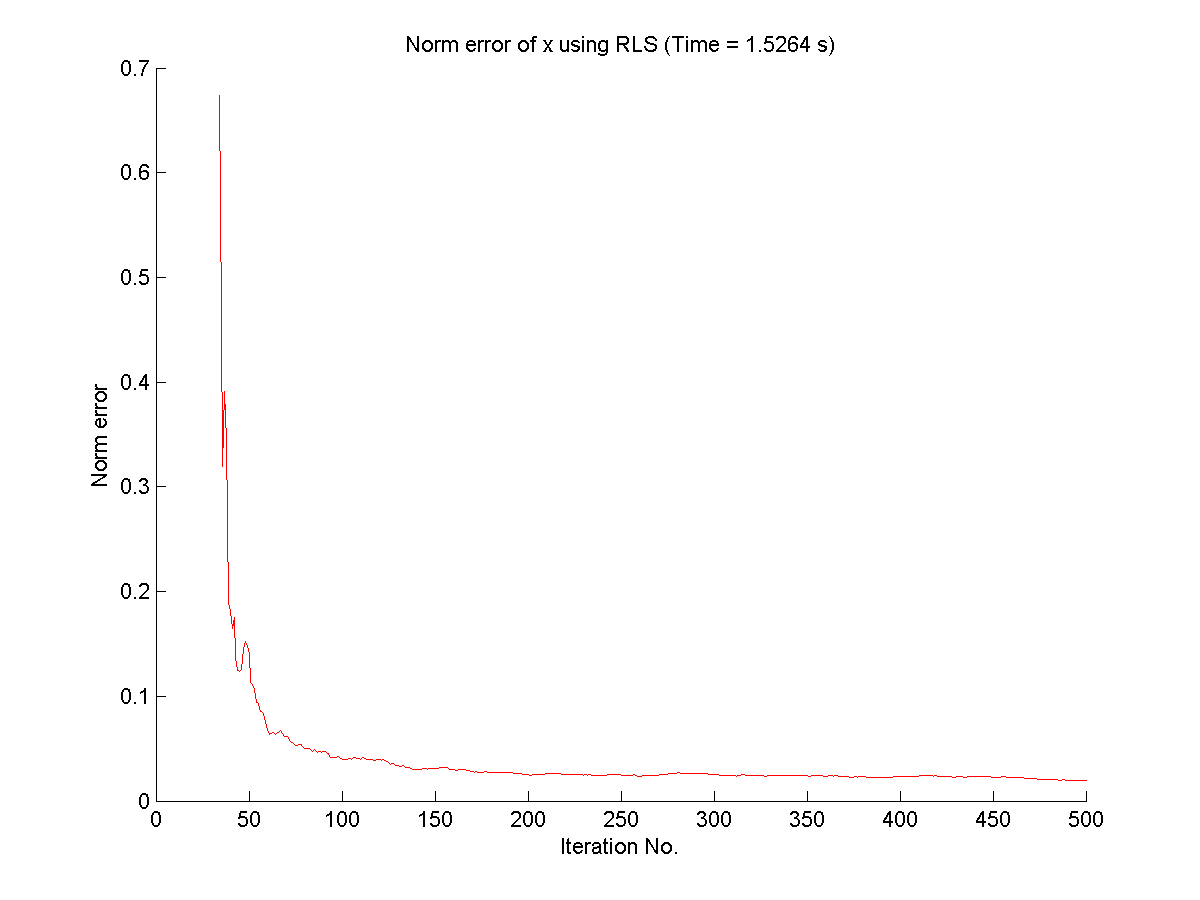
\includegraphics[width=0.7\textwidth]{Prob4(c).png}
		\setlength{\abovecaptionskip}{0pt} 
		%\caption{Naive Estimate}
		\label{fig:Prob4c}
	\end{minipage}
\end{figure}

\item \textbf{}
\begin{figure}[h!]
	\begin{minipage}[t]{\linewidth}
		\centering
		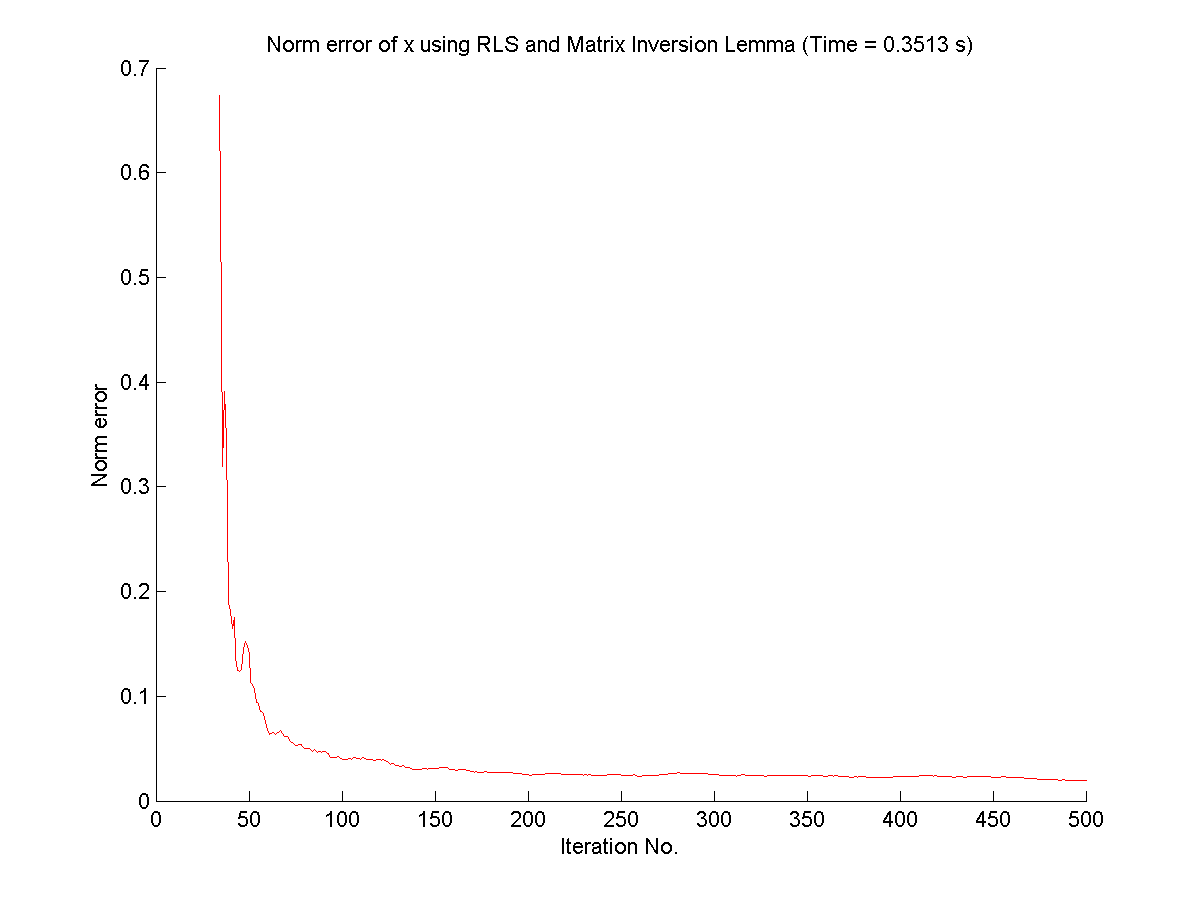
\includegraphics[width=0.7\textwidth]{Prob4(d).png}
		\setlength{\abovecaptionskip}{0pt} 
		%\caption{Naive Estimate}
		\label{fig:Prob4d}
	\end{minipage}
\end{figure}

\end{enumerate}
%Prob. 5  Forgetting factor or exponential windowing
\noindent \textbf{Problem  5:}
\begin{enumerate}
\setlength{\itemsep}{.1in}
\renewcommand{\labelenumi}{(\alph{enumi})}
\item We need to find $n$ such that rank $A_n=20$, the dimension of $x$. This requires that the number of rows in $\text{rows of}~A_n \ge20$, thus the minimal $n$ is 7. We check that indeed the rank of $A_{7}$ is $20$.

\item \textbf{}
\begin{figure}[h!]
	\begin{minipage}[t]{\linewidth}
		\centering
		
\includegraphics[width=0.7\textwidth]{Prob5(b).png}
		\setlength{\abovecaptionskip}{0pt} 
		%\caption{Naive Estimate}
		\label{fig:Prob5b}
	\end{minipage}
\end{figure}

\item \textbf{}
\begin{figure}[h!]
	\begin{minipage}[t]{\linewidth}
		\centering
		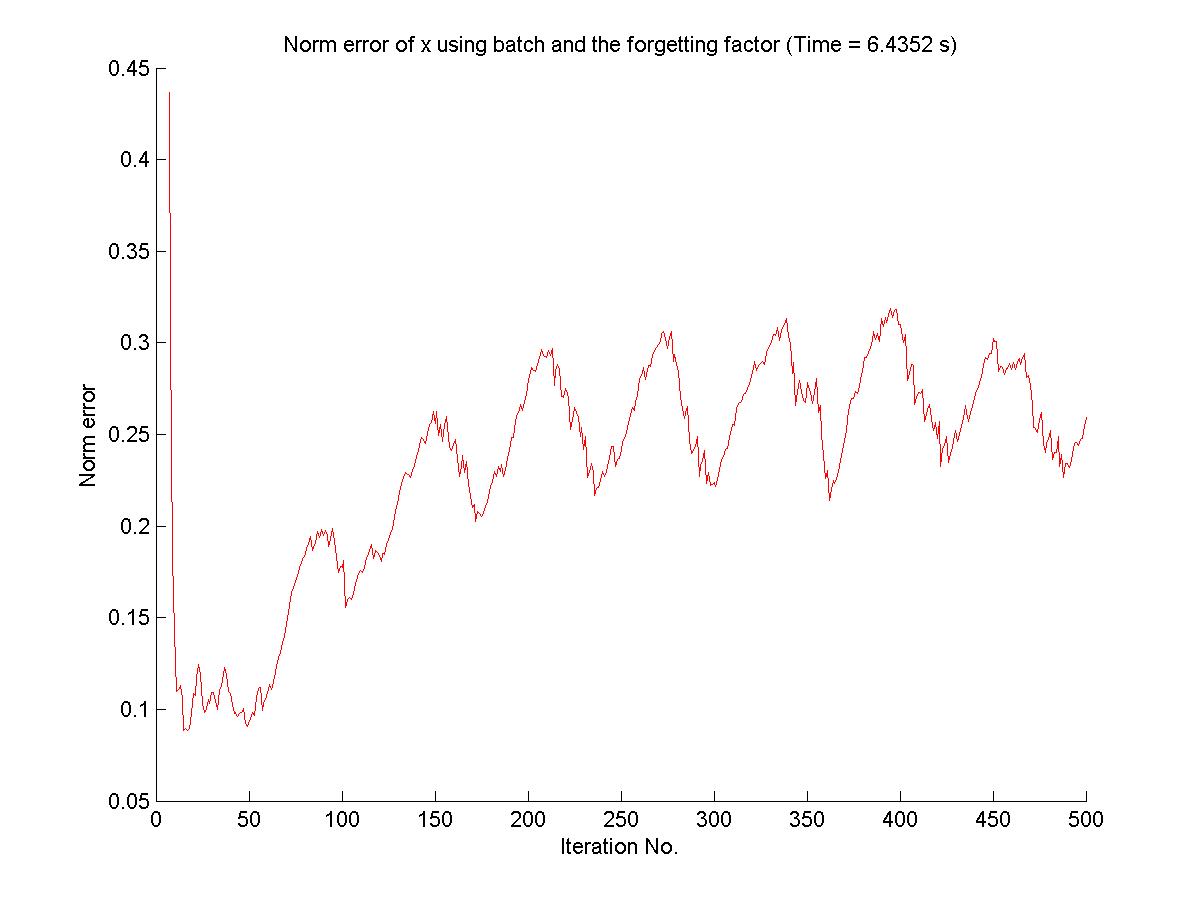
\includegraphics[width=0.7\textwidth]{Prob5(c).png}
		\setlength{\abovecaptionskip}{0pt} 
		%\caption{Naive Estimate}
		\label{fig:Prob5c}
	\end{minipage}
\end{figure}

\item \textbf{}
\begin{figure}[h!]
	\begin{minipage}[t]{\linewidth}
		\centering
		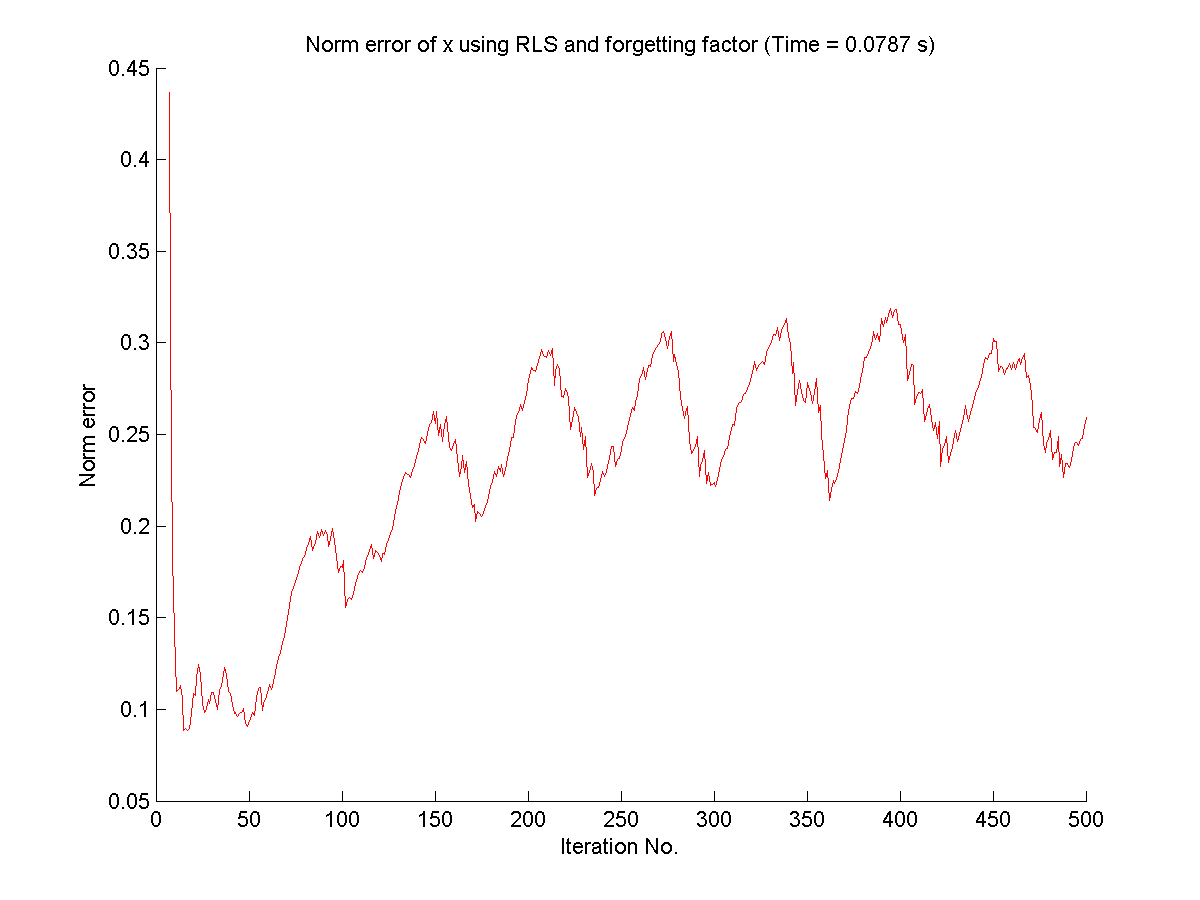
\includegraphics[width=0.7\textwidth]{Prob5(d).png}
		\setlength{\abovecaptionskip}{0pt} 
		%\caption{Naive Estimate}
		\label{fig:Prob5d}
	\end{minipage}
\end{figure}
\newpage
\end{enumerate}
%Prob. 6  Data Association: Mahalanobis Distance
\noindent \textbf{Problem  6:}
\begin{enumerate}
	\item[(a)] Using Euclidean Distance
\begin{enumerate}
	\item[(i)] $ d_{Euc}(P_1 , \mu_{S_1}) = \Vert \begin{bmatrix} 4 \\ 2\end{bmatrix} - \begin{bmatrix} 4 \\ 0\end{bmatrix} \Vert_2 ~=~ \Vert \begin{bmatrix} 0 \\ 2\end{bmatrix} \Vert_2 ~=~~~ 2$	\\ \vskip 1mm

	$ d_{Euc}(P_1 , \mu_{S_2}) = \Vert \begin{bmatrix} 4 \\ 2\end{bmatrix} - \begin{bmatrix} 0 \\ 2\end{bmatrix} \Vert_2 ~=~ \Vert \begin{bmatrix} 4 \\ 0\end{bmatrix} \Vert_2 ~=~~~ 4$ \\ \vskip 1mm
	$\therefore C(P_1) = 1$
	
	\item[(ii)] $ d_{Euc}(P_2 , \mu_{S_1}) = \Vert \begin{bmatrix} 2.8 \\ 1\end{bmatrix} - \begin{bmatrix} 4 \\ 0\end{bmatrix} \Vert_2 ~=~ \Vert \begin{bmatrix} -1.2 \\ 1\end{bmatrix} \Vert_2 ~=~~~ 1.562$	\\ \vskip 1mm
	$ d_{Euc}(P_2 , \mu_{S_2}) = \Vert \begin{bmatrix} 2.8 \\ 1\end{bmatrix} - \begin{bmatrix} 0 \\ 2\end{bmatrix} \Vert_2 ~=~ \Vert \begin{bmatrix} 2.8 \\ -1\end{bmatrix} \Vert_2 ~=~~~ 2.9732$ \\ \vskip 1mm
	$\therefore C(P_2) = 1$

	\item[(iii)] $ d_{Euc}(P_3 , \mu_{S_1}) = \Vert \begin{bmatrix} 2 \\ 0\end{bmatrix} - \begin{bmatrix} 4 \\ 0\end{bmatrix} \Vert_2 ~=~ \Vert \begin{bmatrix} -2 \\ 0\end{bmatrix} \Vert_2 ~=~~~ 2$	\\ \vskip 1mm
	$ d_{Euc}(P_3 , \mu_{S_2}) = \Vert \begin{bmatrix} 2 \\ 0\end{bmatrix} - \begin{bmatrix} 0 \\ 2\end{bmatrix} \Vert_2 ~=~ \Vert \begin{bmatrix} 2 \\ -2\end{bmatrix} \Vert_2 ~=~~~ 
	2.8284$ \\ \vskip 1mm
	$\therefore C(P_3) = 1$
\end{enumerate}

\item[(b)] Using Mahalanobis Distance
\begin{align}
	\Sigma^{-1}_{S_1} = \begin{bmatrix}
		4 & 0 \\ 0 & 0.5
	\end{bmatrix},~~~ \Sigma^{-1}_{S_2} = \begin{bmatrix}
	0.25 & -0.25 \\ -0.25 & 0.75
	\end{bmatrix}
	\nonumber
\end{align}
\begin{enumerate}
	\item[(i)] $ d_{M}(P_1 , \mu_{S_1}) = \Vert \begin{bmatrix} 4 \\ 2\end{bmatrix} - \begin{bmatrix} 4 \\ 0\end{bmatrix} \Vert_{\Sigma^{-1}_{S_1}} ~=~ \Vert \begin{bmatrix} 0 \\ 2\end{bmatrix} \Vert_{\Sigma^{-1}_{S_1}} ~=
	~ \sqrt{[0 ~~ 2] \begin{bmatrix}4 & 0 \\ 0 & 0.5\end{bmatrix} \begin{bmatrix}0 \\ 2 \end{bmatrix}} ~=~~1.4142$	\\ \vskip 1mm	
	$ d_{M}(P_1 , \mu_{S_2}) = \Vert \begin{bmatrix} 4 \\ 2\end{bmatrix} - \begin{bmatrix} 0 \\ 2\end{bmatrix} \Vert_{\Sigma^{-1}_{S_2}} ~=~ \Vert \begin{bmatrix} 4 \\ 0\end{bmatrix} \Vert_{\Sigma^{-1}_{S_2}} ~=
	~ \sqrt{[4 ~~ 0] \begin{bmatrix}0.25 & -0.25 \\ -0.25 & 0.75\end{bmatrix} \begin{bmatrix}4 \\ 0 \end{bmatrix}} ~=~~ 2$	\\ \vskip 1mm
	$\therefore C(P_1) = 1$
	
	\item[(ii)] $ d_{M}(P_2 , \mu_{S_1}) = \Vert \begin{bmatrix} 2.8 \\ 1\end{bmatrix} - \begin{bmatrix} 4 \\ 0\end{bmatrix} \Vert_{\Sigma^{-1}_{S_1}} ~=~ \Vert \begin{bmatrix} -1.2 \\ 1\end{bmatrix} \Vert_{\Sigma^{-1}_{S_1}} ~=
	~ \sqrt{[-1.2 ~~ 1] \begin{bmatrix}4 & 0 \\ 0 & 0.5\end{bmatrix} \begin{bmatrix}-1.2 \\ 1 \end{bmatrix}} ~=~~2.5020$	\\ \vskip 1mm	
	$ d_{M}(P_2 , \mu_{S_2}) = \Vert \begin{bmatrix} 2.8 \\ 1\end{bmatrix} - \begin{bmatrix} 0 \\ 2\end{bmatrix} \Vert_{\Sigma^{-1}_{S_2}} ~=~ \Vert \begin{bmatrix} 2.8 \\ -1\end{bmatrix} \Vert_{\Sigma^{-1}_{S_2}} ~=
	~ \sqrt{[2.8 ~~ -1] \begin{bmatrix}0.25 & -0.25 \\ -0.25 & 0.75\end{bmatrix} \begin{bmatrix}2.8 \\ -1 \end{bmatrix}} ~=~~ 2.0273$	\\ \vskip 1mm
	$\therefore C(P_2) = 2$
	
	\item[(ii)] $ d_{M}(P_3 , \mu_{S_1}) = \Vert \begin{bmatrix} 2 \\ 0\end{bmatrix} - \begin{bmatrix} 4 \\ 0\end{bmatrix} \Vert_{\Sigma^{-1}_{S_1}} ~=~ \Vert \begin{bmatrix} -2 \\ 0\end{bmatrix} \Vert_{\Sigma^{-1}_{S_1}} ~=
	~ \sqrt{[-2 ~~ 0] \begin{bmatrix}4 & 0 \\ 0 & 0.5\end{bmatrix} \begin{bmatrix}-2 \\ 0 \end{bmatrix}} ~=~~4$	\\ \vskip 1mm
		
	$ d_{M}(P_3 , \mu_{S_2}) = \Vert \begin{bmatrix} 2 \\ 0\end{bmatrix} - \begin{bmatrix} 0 \\ 2\end{bmatrix} \Vert_{\Sigma^{-1}_{S_2}} ~=~ \Vert \begin{bmatrix} 2 \\ -2\end{bmatrix} \Vert_{\Sigma^{-1}_{S_2}} ~=
	~ \sqrt{[2 ~~ -2] \begin{bmatrix}0.25 & -0.25 \\ -0.25 & 0.75\end{bmatrix} \begin{bmatrix} 2 \\ -2 \end{bmatrix}} ~=~~ 2.4495$	\\ \vskip 1mm
	
	$\therefore C(P_3) = 2$
	
\end{enumerate}

\end{enumerate}
\end{document}




